\documentclass[a4paper]{article}


\usepackage{alphabeta} 
\usepackage{enumitem} 
\usepackage{mathtools}
\usepackage{amsmath, amssymb} 
\usepackage{amsthm}
\usepackage{cancel} 
\usepackage[margin=0.70in]{geometry} 
\geometry{left=3cm,right=3cm,top=2.4cm,bottom=2.4cm}	%the page geometry as defined, A4=210x297mm
\usepackage{graphicx}
\usepackage{wrapfig}
\usepackage[center]{caption}
\usepackage{textcomp}
\usepackage{tabto}
\usepackage{layout}
\usepackage{bm}
\usepackage{minipage-marginpar}
\usepackage[dvipsnames]{xcolor}
\usepackage{hyperref}
\usepackage{dutchcal}
\usepackage{derivative}
\usepackage{esint}
%\usepackage{biblatex}
\usepackage{subcaption}
\usepackage{booktabs}\usepackage{derivative}
\usepackage[flushleft]{threeparttable}
\usepackage[capbesideposition=outside,capbesidesep=quad]{floatrow}
\usepackage{derivative}
\usepackage[thinc]{esdiff}
\usepackage{lipsum}
\usepackage{arydshln}
%%RENEW

\newtheorem{problem}{Άσκηση}
\newtheorem*{solution*}{Λύση}
\newtheorem{definition}{Ορισμός}[subsection]
\newtheorem{properties}{Ιδιότητες}[subsection]
\newtheorem{theorem}{Θεώρημα}[subsection]
\newtheorem{protash}{Πρόταση}[subsection]
\newtheorem{porisma}{Πόρισμα}[subsection]
\newtheorem{lemma}{Λήμμα}[subsection]
\newtheorem*{prooof}{Απόδειξη}
\newtheorem*{notes}{Παρατηρήσεις}
\newtheorem*{note}{Παρατήρηση}
\newtheorem*{app}{Εφαρμογή} 
\newtheorem*{example}{Παράδειγμα}
\newtheorem*{examples}{Παραδείγματα}


\newcommand\numberthis{\addtocounter{equation}{1}\tag{\theequation}}
%\renewcommand{\labelenumi}{\roman{enumi}}
\newcommand{\approxtext}[1]{\ensuremath{\stackrel{\text{#1}}{\approx}}}
\renewcommand{\figurename}{Εικόνα.}
\renewcommand{\tablename}{Πίνακας.}
%\renewcommand\refname{New References Header}
\renewcommand*\contentsname{Περιεχόμενα}
%\DeclareDerivative{\odv}{\mathrm{d}}


\begin{document}
\begin{titlepage}			%makes a title page. Remember to change the author, CID, username and group number to what is appropriate for you!
	\centering
	{\scshape\LARGE Εθνικό Μετσόβιο Πολυτεχνείο\par}
	{\scshape \LARGE Σ.Ε.Μ.Φ.Ε.\par}
	\vspace{1cm}
	{\huge\bfseries Διοδικό Laser\par}
	\vspace{1cm}
	{\Large\itshape Θωμόπουλος Σπύρος\par}		%remember to change these!
	
	%		{\large Group \@group\unskip\strut\par}
	{\large spyros.thomop@gmail.com/ ge19042@mail.ntua.gr\par \hfill \\}% 		%remember to change these!
	\vspace{1cm}
	{\large Ημερμονηνία Παράδοσης 09/05/2022\par}
\end{titlepage}

\subsection*{Σκοπός}

	Ο σκοπός της εν λόγω εργαστηριακής άσκησης είναι αρχικά να σταθεροποιήσουμε το ρεύμα σε ένα τροφοδοτικό που χρησιμοποιείται σε διοδικό laser και έπειτα να μελετήσουμε κάποιες βασικές ιδιότες αυτών των laser σχετικά με το ρεύμα κατωφλίου και την ευθυγράμμιση.

\subsection*{Θεωρητικά Στοιχεία}


	Για την κατασκευή ενός διοδικού laser έχουμε φέρει σε επαφή δύο ημιαγωγούς, έναν τύπου P με περίσσεια θετικών φορτίων (οπές) και έναν τύπου N με περίσσεια αρνητικών φορτίων (ηλεκτρόνια), αυτή ονομάζεται επαφή PN. Στην περιοχή επαφής των δύο ημιαγωγών δημιουργείται μία διαφορά δυναμικού και ένας χώρος όπου υπάρχουν ταυτόχρονα ηλεκτρόνια και οπές. Κάθε φορά που ένα ηλεκτρόνιο έρχεται σε επαφή με μία οπή έχουμε εκπομπή ενός φωτονίου. Όπως και στα laser αερίου θέλουμε να επιτύχουμε εξαναγκασμένη εκπομπή και για να λειτουργήσει αντιστροφή πληθυσμών, η οποία επιτυγχάνεται όταν τα ηλεκτρόνια στην ζώνη αγωγιμότητας είναι περισσότερα από τις οπές της ζώνης σθένους πράγμα που συμβαίνει από μία συγκεκριμένη τιμή του ρεύματος τροφοδοσίας και πάνω (τιμή κατωφλίου $I_{thr}$).
	
	Ωστόσο, επειδή η εν λόγω τιμή είναι αυστηρά καθορισμένη, όταν το ρεύμα γίνει λίγο μικρότερο από αυτή τότε σταματάει η λειτουργία της διόδου ως laser, άρα για να έχουμε μία σταθερή λειτουρία θα πρέπει να έχουμε και σταθερή τιμή του ρεύματος. Για να το επιτύχουμε αυτό χρησιμοποιούμε έναν \textit{τελεστικό ενισχυτή}. Ο τελεστικός ενισχυτής έχει δύο εισόδους, μία μη-αναστρέφουσα ''+'' ($\Delta\phi =\pi$με έξοδο) και μία αναστρέφουσα ''-'' ($\Delta\phi = 0$ με έξοδο) και δίνει στην έξοδο μία ενισχυμένη και σταθερή τάση δεχόμενος τις 2 μεταβλητές.
 	
 	Τέλος, η απόκλιση της δέσμης του διοδικού laser είναι διαφορετική στους δύο άξονές της και συγκεκριμένα μεγαλύτερη στον άξονα y και αυτό θα μελετηθεί στο τελευταίο κομμάτι της άσκησης.
 	
\subsection*{Πειραματική Διάταξη}
	Η πειραματική διάταξη αποτελείται από: 
		\begin{enumerate}
			\item \textbf{Μέρος Α}
				\begin{itemize}
					\item[.] Τροφοδοτικά τάσεων $E_A (10V)$ σταθερή, $E_B(15V)$  ρυθμιζόμενη
					\item[.] Αμπερόμετρο
					\item[.] Βολτόμετρο
					\item[.] Δίοδο LED
					\item[.] Ποτενσιόμετρο
					\item[.] Πλακέτα
					\item[.] 3 Αντιστάσεις 
					\item[.] Τρανζίστορ 
					\item[.] Τελεστικός ενισχυτής
				\end{itemize}
				\begin{figure}[h!]
					\centering
					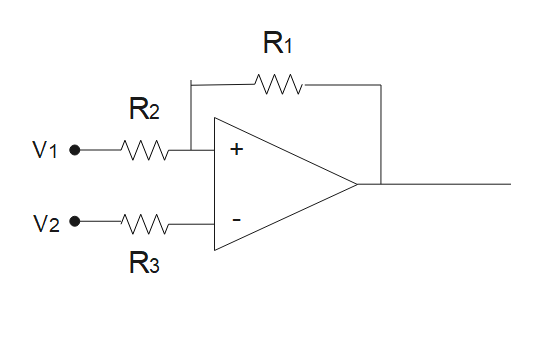
\includegraphics[scale=0.4]{oper.png}
					\caption{Τελεστικός ενισχυτής }
					\label{im1}
				\end{figure}
		
				Η πηγή $E_B$ τροφοδοτεί την δίοδο, όμως λόγω τυχών μεταβολών του ρεύματος που παρέχει, παρεμβάλλουμε έναν τελεστικό ενισχυτή ο οποίος δέχεται δύο τάσεις εισόδου $V_1$ (σταθερή) από το ποτενσιόμετρο και $V_2$ και διατηρεί τις $V_1$, $V_2$ ίσες δίνοντας μία ενισχυμένη τάση στην έξοδο η οποία μεταβάλλει την αγωγιμότητα του ημιαγωγού στο τρανζίστορ έτσι ώστε να παραμένει σταθερό το ρεύμα εξόδου.				
				
		
			\item \textbf{Μέρος Β}
				\begin{itemize}
					\item[.] Διοδικό Laser 30mW μήκους κύματος $670nm$
					\item[.] Ρυθμιζόμενο τροφοδοικό 
					\item[.] Στηρίγματα εξαρτημάτων laser 
					\item[.] Φωτοανιχνευτής   
				\end{itemize}
%			Η διάταξη φαίνεται στην παρακάτω Εικόνα 
%				\begin{figure}[h!]
%					\centering
%					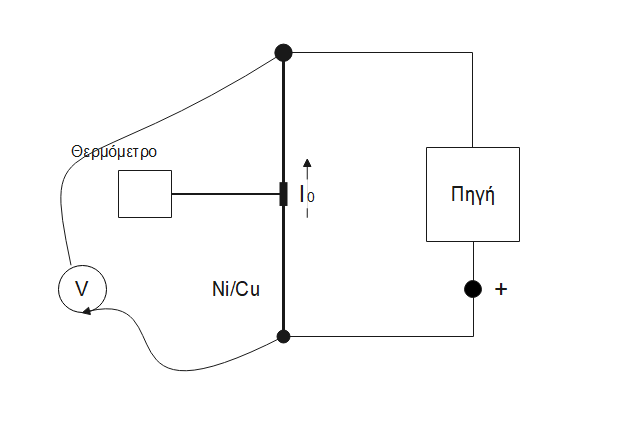
\includegraphics[width=0.7\linewidth]{setup.png}
%				\end{figure}
		
			\item \textbf{Μέρος Γ}
				\begin{itemize}
					\item[.]  Διοδικό Laser 30mW μήκους κύματος $670nm$
					\item[.]  Ρυθμιζόμενο τροφοδοικό
					\item[.]  Φωτοανιχνευτής
					\item[.] Pinhole
					\item[.]  Στηρίγματα εξαρτημάτων Laser 
				\end{itemize}
		
		\end{enumerate}
	\vspace{-0.6cm}
\subsection*{Πειραματική Διαδικασία - Επεξεργασία Μετρήσεων}
	\subsubsection*{Μέρος Α}
	Ρυθμίζουμε την τάση $E_B=10V$, μεταβάλλουμε την $V_1$ από $0-4.5V$ με βήμα 0.5V και μετράμε την $V_2$ στα άκρα της αντίστασης $R_3$.
	Τα αποτελέσματα φαίνονται στον Πίνακα (\ref{mat1}) 
		\begin{table}[h!]
			\centering
			\begin{tabular}{r|r}
				$V_1(V)$ & $V_2(V)$ \\ \hline\hline
				 0.47&0.48\\
				1.01&1.51\\
				1.51&1.51\\
				2.00&2.00\\
				2.50&2.50\\
				3.00&3.06\\
				3.50&3.50\\
				4.00&4.00\\
				4.50&4.22			
			\end{tabular}
			\caption{ }
			\label{mat1}
		\end{table}
		
		Η γραφική παράσταση φαίνεται στην Εικόνα (\ref{im2}), όπου και παρατηρούμε μερικά σήμεία στα οποία οι δύο τάσεις δεν ταυτίζονται. Αυτό ίσως οφείλεται σε δική μας αστοχία στην μέτρηση.
		
		\begin{figure}[h!]
			\centering
			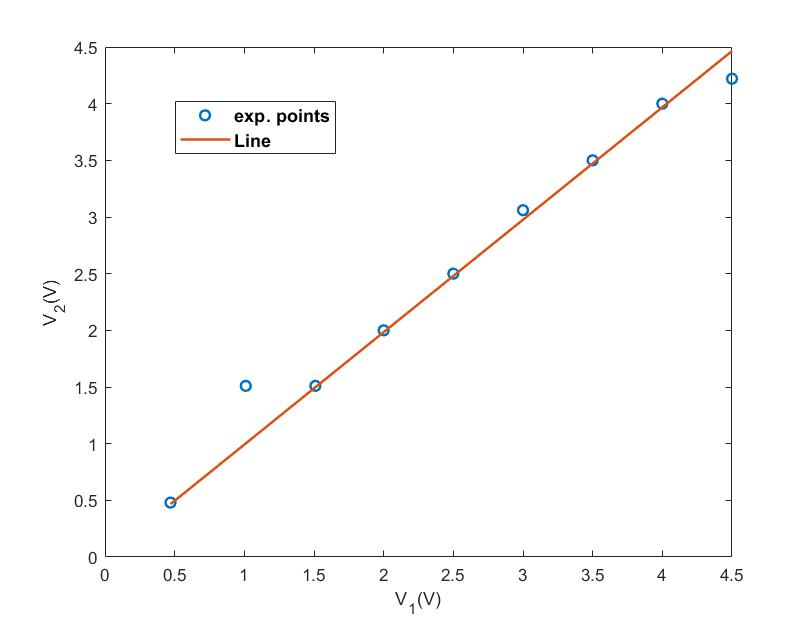
\includegraphics[width=0.65\linewidth]{plot1.jpg}
			\caption{$V_1-V_2$ }
			\label{im2}
		\end{figure}
		
		
		Τώρα ρυθμίζουμε το ποτενσιόμετρο ώστε να δίνει ρεύμα $I_A=40mA$, μεταβάλλουμε την $E_B$ από $8-12V$ με βήμα 0.5V και μετράμε το ρεύμα στην έξοδο του τελεστικού ενισχυτή. Έπειτα επαναλαμβάνουμε για $I_B=45mA$ και $I_C = 50mA$. Τα ποτελέσματα φαίνονται στον Πίνακα (\ref{mat2}) και η γραφική παράσταση στην Εικόνα (\ref{im3}): 
		\begin{table}[h!]
			\centering
			\begin{tabular}{r|r|r|r}
				$E_B$(V) & $I_A(nA)$ & $I_B(mA)$ & $I_C(mA)$ \\\hline\hline
				8.0&40&45&50\\
				8.5&40&45&50\\
				9.0&40&45&50\\
				9.5&40&45&50\\
				10.0&40&45&50\\
				10.5&40&45&50\\
				11.5&40&45&50\\
				11.5&40&45&50\\
				12.0&40&45&50
			\end{tabular}
			\caption{ }
			\label{mat2}
		\end{table}
		 
		 
		 \begin{figure}[h!]
		 	\centering
		 	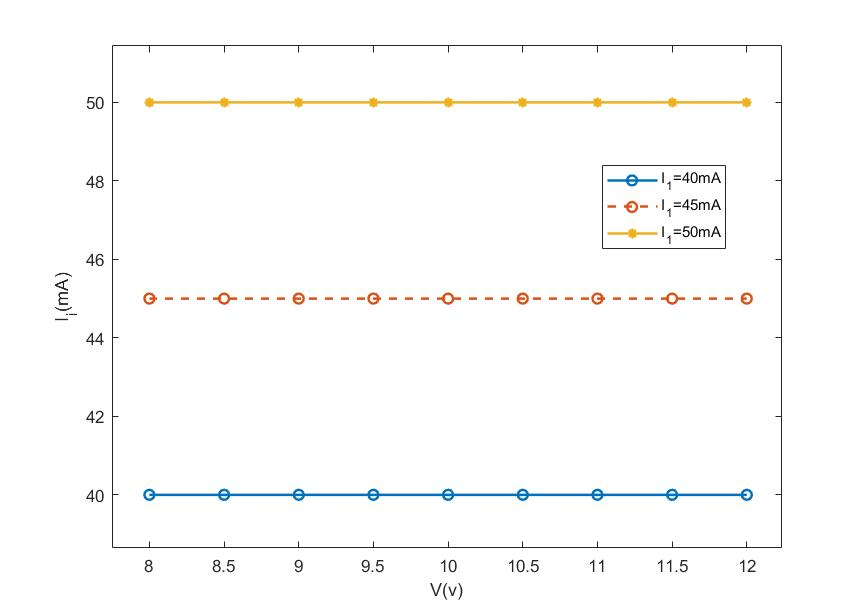
\includegraphics[width=0.7\linewidth]{plot2.jpg}
		 	\caption{ }
		 	\label{im3}
		 \end{figure}
		 
		 Τώρα διατηρώντας το ρεύμα στα $I=40mA$ μεβάλλουμε την τάση της πηγής $E_B$ από 8-12V με βήμα 0.5V και μετράμε τις τάσεις $V_2$ και $V_3$. Τα αποτελέσματα φαίνονται στον Πίνακα (\ref{mat3}) και η γραφική στην Εικόνα (\ref{im4}).
		 \begin{table}[h!]
		 	\centering
		 	\begin{tabular}{r|r|r}
		 		$E_B(V)$ & $V_2(V)$ & $V_3(V)$ \\\hline\hline
		 		8.0&4.05&1.23 \\
				8.5&4.04&1.61\\
				9.0&4.10&2.12\\
				9.5&4.13&2.51\\
				10.0&4.18&3.20\\
				10.5&4.22&3.86\\
				11.0&4.25&4.50\\
				11.5&4.28&5.04\\
				12.0&4.81&5.43		 	
		 	\end{tabular}
		 	\caption{ }
		 	\label{mat3}
		 \end{table}
		 
		 \begin{figure}[h!]
		 	\centering
		 	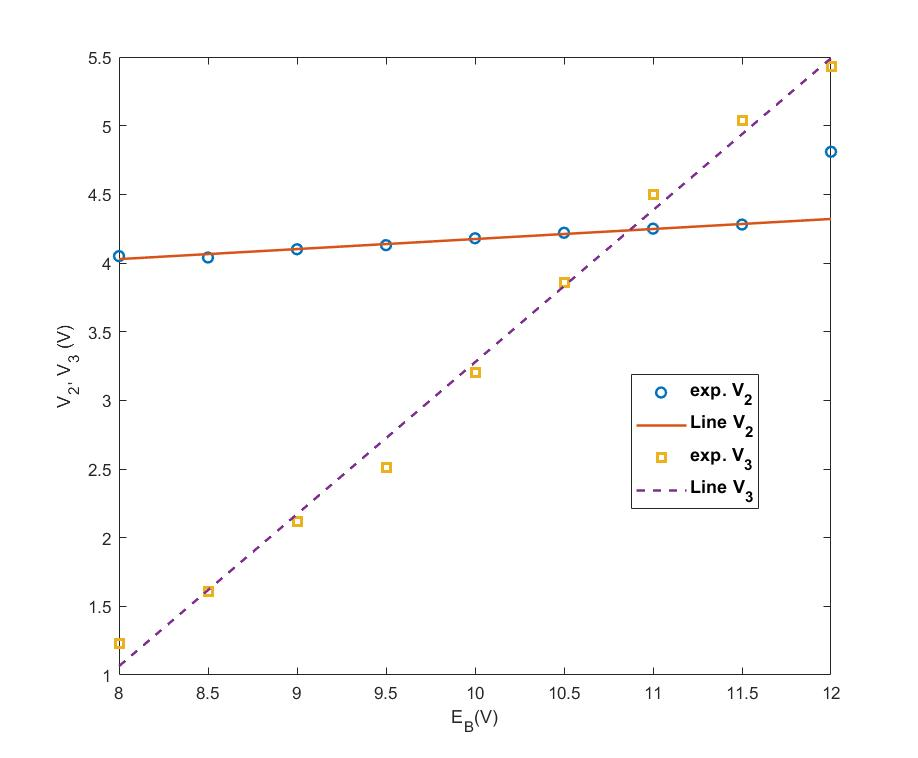
\includegraphics[width=0.7\linewidth]{plot3.jpg}
		 	\caption{Για το σχεδιασμό της Ευθείας για το $V_2$ δεν έχω συμπεριλάβει το τελευταίο σημείο.}
		 	\label{im4}
		 \end{figure}
		 \newpage
		 
	\subsubsection*{Μέρος Β}
		Αυξάνουμε σιγά σιγά το ρεύμα τροφοδοσίας του Laser από 0-35mA και ευθυγραμμίζουμε την διάταξη, προσδιορίζοντας την θέση όπου ελαχιστοποιείται η κηλίδα του laser. Τώρα μεταβάλλουμε το ρεύμα τροφοδοσίας του laser από 0-50mA με βήμα 5mA και καταγράφουμε την τιμή της τάσης στον μετρητή ισχύος. Επίσης, με την σχέση βαθμονόμησης του ισχυομέτρου $P[mW] = -4.8979 + 18.4843x[V] $, μετατρέπουμε την τάση σε ισχύ. Τα αποτελέσματα φαίνονται στον Πίνακα (\ref{mat4}) και η γραφική παράσταση στην Εικόνα (\ref{im5}), όπου και παρατηρούμε πως υπάρχει μία τιμή της τάσης $V_1$ πάνω από την οποία αυξάνεται απότομα η ισχύς του laser.
		\begin{table}[h!]
			\centering
			\begin{tabular}{r|r|r}
				$V_1(mV)$ & V(V) & P(mW) \\\hline\hline
				4.7&0.34&82\\
4.9&0.34&85.7\\
5.1&0.34&89.4\\
5.2&0.38&91.2\\
5.4&0.38&94.9\\
6.3&0.38&111.6\\
23.7&0.39&433.2\\
25.2&0.39&460.9\\
28.2&0.4&516.4\\
29.5&0.4&540.4\\
31.6&0.4&579.2\\
32.7&0.41&599.5\\
33.9&0.42&621.7\\
35.2&0.45&645.7\\
40.5&0.5&743.7\\
45.7&0.52&839.8\\
49.8&0.53&915.6			
			\end{tabular}
			\caption{ }
			\label{mat4}
		\end{table}
	
	\begin{figure}[h!]
		\centering
		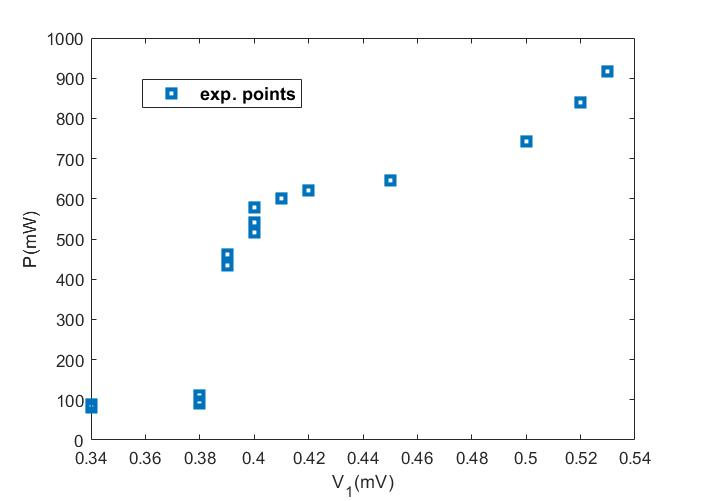
\includegraphics[width=0.8\linewidth]{plot4.jpg}
		\caption{ }
		\label{im5}
	\end{figure}
	
	
	\subsubsection*{Μέρος Γ}
		Θέτουμε την τάση στην τροφοδοσία του Laser στα 48mV και ευθυγραμμίζουμε την διάταξη έτσι ώστε καθώς η δέσμη περνάει μεσα από το εμπόδιο να παίνρουμε την μέγιστη ένδειξη. Στρίβουμε την μικρομετρική βίδα που μετακινεί το εμπόδιο κατά το άξονα x και αφού το ξαναευθυγραμμίσουμε στρίβουμε την βίδα του άξονα y. Τα αποτελέσματα φαίνονται στον Πίνακα (\ref{mat5}) και η γραφική παράσταση στην Εικόνα (\ref{im6}).
		
		\begin{table}[h!]
			\centering
			\begin{tabular}{r|r||r|r}
				Βήμα x & $V_2(mV)$ & Βήμα y & $V_{2}(mV)$ \\\hline\hline
				0&0.52&0&0.52\\
1&0.51&1&0.52\\
2&0.47&2&0.52\\
3&0.44&3&0.52\\
4&0.42&4&0.52\\
5&0.40&5&0.52\\
6&0.39&6&0.52\\
-&-&7&0.52\\
-&-&8&0.52\\
-&-&9&0.52\\
-&-&10&0.52\\
-&-&11&0.52\\
-&-&12&0.52\\
-&-&13&0.52\\
-&-&14&0.52\\
-&-&15&0.52\\
-&-&16&0.52\\
-&-&17&0.52\\
-&-&18&0.52\\
-&-&19&0.52\\
-&-&20&0.52\\
-&-&21&0.52\\
-&-&22&0.51\\
-&-&23&0.45\\
-&-&24&0.42\\
-&-&25&0.39\\
-&-&26&0.39\\
-&-&27&0.37\\
-&-&28&0.36\\
-&-&29&0.35\\
-&-&30&0.34				
			\end{tabular}
			\caption{ }
			\label{mat5}
		\end{table}
		
	\begin{figure}[h!]
		\centering
		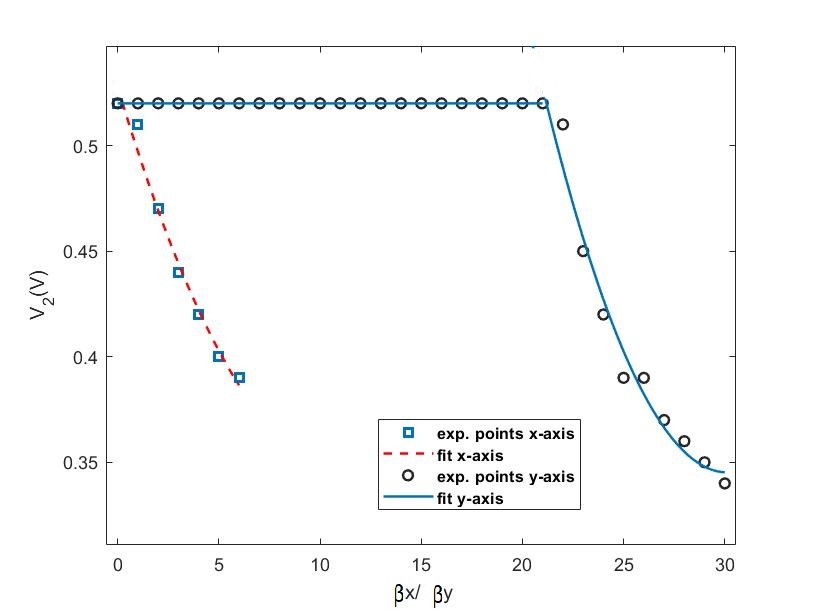
\includegraphics[scale=0.7]{plot5.jpg}
		\caption{ }
		\label{im6}
	\end{figure}
	
	Παρατηρούμε ότι για τον y άξονα, η τάση που ανιχνεύουμε δεν πέφτει από την αρχή της μετακίνησης της οπής σε αντίθεση με την μετακίνηση κατά τον άξονα x.
\end{document}